\chapter{Related Works}

\section{Learning cellular automaton dynamics}

\noindent
\textbf{Learning Cellular Automaton Dynamics with Neural Networks} (Wulff and Hertz, 1992) \cite{wulff1992learning} is a seminal work in this area.
It uses a lattice-shaped network with the same structure as the CA being simulated.
Each node in this lattice is a Probabilistic Logic Node, also known as a $\Sigma-\Pi$ unit \cite{gurney1992training}.
These units are capable of representing any boolean function.
That is to say $ \forall f: \mathbb{R}^N \to \{-1, 1\}, \exists~w_1, w_2, ... , w_N \in \R $ such that,

\begin{equation} \label{eq:sigma_pi}
f(S_1, S_2, ..., S_N) = sgn\left[ \sum_{j=1}^{N} w_j \prod_{i \in I_j} S_i(t) \right]
\end{equation}

\noindent
where index set $I_j$ is randomly drawn from the integers $\{1, 2, ..., N\}$ without replacement.
Notably, these units do not require input from every neighbour to learn successfully.
In fact, this paper found any index set of size $|I_j| \geq \frac{N}{2}$ to be sufficient.
This insight significantly reduced training time.\\ 
3 learning goals were established for the network.
In order of increasing difficulty they were:

\begin{enumerate}
  \item Extrapolation: Learn to simulate a CA for a \textit{particular} initial condition at any time
  \item Dynamics : Learn to simulate a CA for \textit{any} initial condition after short-lived patterns have been exhausted
  \item Full Rule : Learn to simulate a CA for any initial condition at any time
\end{enumerate}

This work was largely concerned with class 3 (chaotic) and class 4 (complex) behaviour. 
All 9 known examples of class 3 1D automata were tested on.
However, at the time, it was believed that 1D CA could not exhibit class 4 behaviour so testing was also conducted on Conway's Game of Life.
There were two settings under which testing was done.
 

\begin{enumerate}
  \item Shared weights: There was a single network learning a single transition rule across the automata.
  \item Individual weights: Each cell was learning its own transition rule based on information available from its local neighbourhood only.
\end{enumerate}

With shared weights, this approach was very promising, with extrapolation and dynamics being very easy in the 1D and 2D cases.
Learning the full rule was much harder with the network only being able to do so for 4 out of the 9 candidates in the 1D case. \\ 

With individual weights, all learning was difficult. 
In the 1D case, extrapolation was still possible for all candidates but dynamics was only possible for a single candidate, rule 22. 
Learning Life was also impossible with the network failing to extrapolate even when given several hundred steps of history.\\ 

As the first notable exploration of learning transition rules with neural networks, this paper demonstrated a method for learning chaotic behaviour in cellular automata.
It also divided class 3 elementary CA into two categories according to how easy it is to learn their underlying rule.
Furthermore, it raised many questions for future research.
The most pertinent is whether these results on a few simple examples generalise to all complex and chaotic CA.\\

However, this work only explored class 3 and 4 CA, presumably because these are the most interesting varieties.
For the goal of morphogenesis, we are more interested in the possibility of learning on class 2 CA.

\section{Using evolutionary algorithms}
Another interesting line of research is the use of evolutionary algorithms to evolve ANNs for CA morphogenesis.\\

\noindent
\textbf{Evolving Self-organizing Cellular Automata Based on Neural Network Genotypes} (Elmenreich and Feh\'erv\'ari, 2011) \cite{elmenreich2011evolving} is an early work in this area.
Each cell in a CA is controlled with an ANN with 9 input nodes, a 6-node hidden layer, and 5 output nodes.
One output node indicates the cell's colour while the others propagate information to the cell's 4-neighbourhood.
The input nodes take in the corresponding information from the cell's 4-neighbourhood as well as the colour of all 4 neighbours.
The last input node takes in the current colour of the cell itself.
Although each cell is instantiated with the same ANN, the internal state of each ANN can adapt independently at each time step.
The evolution procedure begins by initialising a population of 100 candidate ANNs with random weights and applying algorithm \ref{alg:ea-ann} repeatedly. 
\begin{algorithm}
\caption{Evolutionary Algorithm to improve ANNs}
\label{alg:ea-ann}
\begin{algorithmic}
\For{\textbf{all} generations}
\For{$i = 0$ to $100$}
\State{Evaluate network $i$ and store score}
\EndFor
\State{Rank networks and create new population as follows:}
\State{Elitism: Select top 15 candidates}
\State{Selection: Randomly select 10 from remainder with a small bias towards fitness and diversity}
\State{Mutations: Copy a randomly selected candidate and mutate its weights and biases. Repeatedly apply this operation until there is a new set of 30 mutated candidates.}
\State{Recombinations: Copy a randomly selected pair of candidates and apply crossover. Repeatedly apply this operation until there is a new set of 40 recombined candidates.}
\State{Concatenate mutated and recombined candidates with the original selected candidates.}
\State{Reinitalise: Initialise 5 new networks with random weights and add to new population}
\EndFor
\end{algorithmic}
\end{algorithm}

Although this work was able to successfully learn simple patterns like flags (\ref{fig:austria-flag}), it failed to learn on more complicated structures like animal skin patterns (\ref{fig:animal-patterns}) or the Mona Lisa (\ref{fig:mona-lisa}).
This is likely due to a poor choice of fitness function given the task at hand.
By comparing pixel-by-pixel, candidates with a largely similar pattern to the reference image in a qualitative sense are scored poorly compared to those that can precisely imitate very small portions of the image.\\

Another problem with evolutionary algorithms, in general, is that they get stuck in suboptimal fitness maxima.
Finally, the broad learning network architecture is flawed because only border cells can infer information about their position in the image.
Since the ratio of inner to outer cells increases for higher resolution images, it gets increasingly difficult to pass this information to central cells.
Therefore this solution is likely to scale poorly as was seen in the 20x29 Mona Lisa case. \\

\begin{figure}[!h]
    \centering
    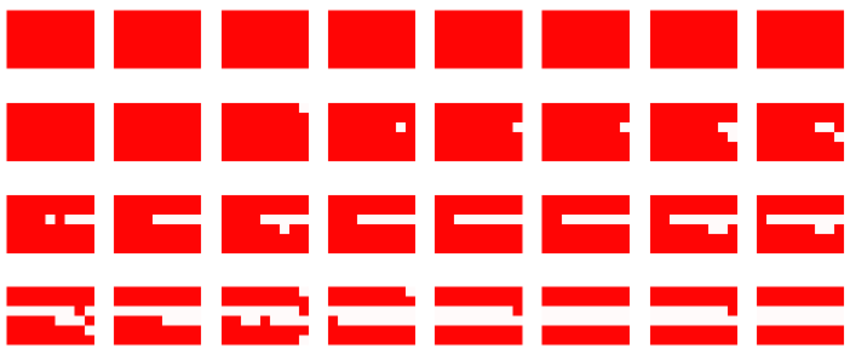
\includegraphics[width=5in]{images/austria-flag.png}
    \caption{Successful reproduction of the Austrian Flag over 90 generations \cite{elmenreich2011evolving}}
    \label{fig:austria-flag}
\end{figure}

\begin{figure}[htp] 
    \centering
    \subfloat[Attempt at learning cow and zebra skin patterns over 300 generations \cite{elmenreich2011evolving}]{%
        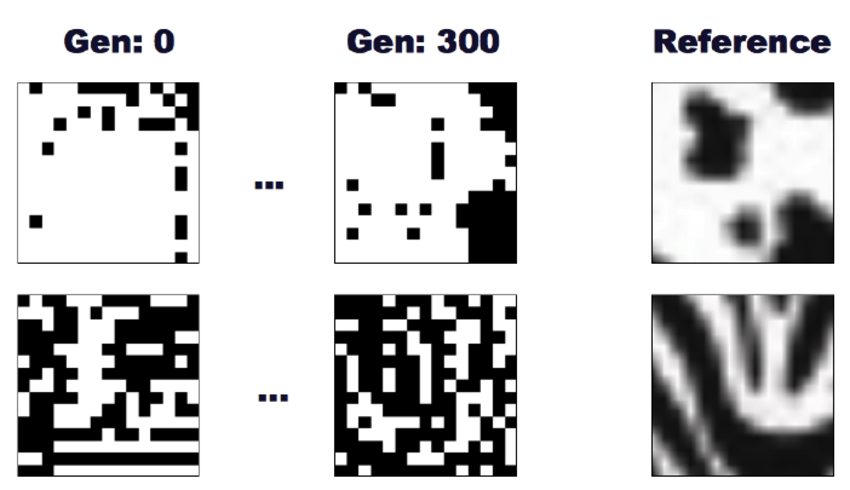
\includegraphics[width=0.45\textwidth]{images/animal-patterns.png}%
        \label{fig:animal-patterns}%
        }%
    \hfill%
    \subfloat[Attempt at learning the Mona Lisa over 500 generations. Depicted from left to right are the original, the reference, and the best reproduction attempt \cite{elmenreich2011evolving}]{%
        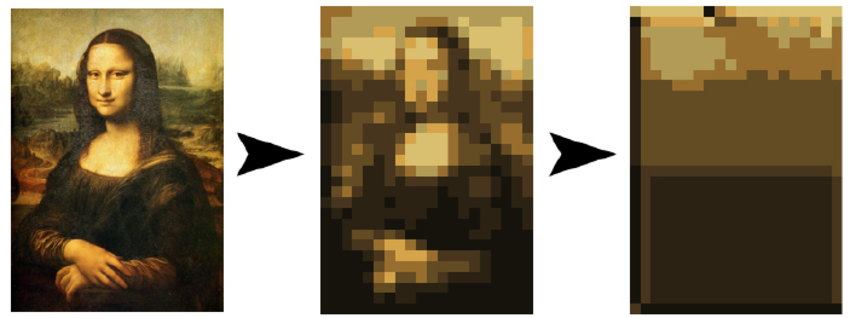
\includegraphics[width=0.45\textwidth]{images/mona-lisa.png}%
        \label{fig:mona-lisa}%
        }%
    \caption{Unsuccessful attempts to learn complex patterns over 300+ generations}
\end{figure}

\raggedbottom
\pagebreak

\noindent
\textbf{CA-NEAT: Evolved Compositional Pattern Producing Networks for Cellular Automata Morphogenesis and Replication} (Nichele et al., 2018) \cite{nichele2017neat} elicited more promising results by opting for a different genotype and evolution strategy.
The genotypes here were compositional pattern producing networks (CPPNs) which were evolved through a neuroevolution of augmenting topologies (NEAT) algorithm.
A CPPN is a type of ANN that is particularly well suited to evolution through genetic algorithms.
Unlike typical ANNs, these networks do not have uniform activation functions across layers.
Instead, a variety of different activation functions are chosen to induce specific patterns in the output.
For example, Gaussian activations are used to create symmetricity and sinusoidal activations are used to create repetition.\\

NEAT is a genetic algorithm designed especially for ANN evolution \cite{stanley2002evolving}.
The initial population consists of simple networks with no hidden layers.
Over multiple generations, nodes and connections are added or disabled.
Activation functions and weights are also adjusted.
As individuals become increasingly dissimilar, a compatibility distance metric is used to segregate individuals into separate species once they cross a threshold of incompatibility.
Pairs for reproduction are only selected within species.
New species are granted a period of immunity during which they won't be eliminated by the algorithm but subsequent poor performance does lead to the removal of failing species to ensure continuous improvement in the fitness of the population.\\

The two goals established by this paper were morphogenesis - to develop a given pattern from a simple seed, and reproduction - to produce at least 3 copies of a pattern from a single instance.
For the purpose of this review, we will focus on the morphogenesis goal.
The fitness function for this is given in equation~\ref{eq:fitness-CPPN}

\begin{align}
\label{eq:fitness-CPPN}
f(x) &= xe^{5(x-1)} \\
\text{where}~x &= \max_{t = 1 .. 30} (r_t)
\end{align}

\noindent
where $r_t$ is the proportion of cells with the correct state at time $t$.
This exponential fitness function suppresses the contribution of dormant cells (i.e. low values of $x$) while maintaining the essential invariant $f(1) = 1$.
This choice biases the algorithm towards more active CA.\\


\begin{figure}[!h]
    \centering
    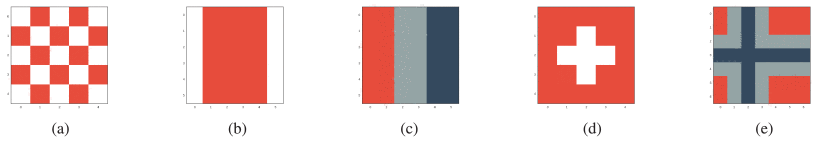
\includegraphics[width=5in]{images/five-flags.png}
    \caption{Five goal patterns for CA-NEAT}
    \caption*{(a) \textit{Mosaic}, (b) \textit{Border}, (c) \textit{Tricolor}, (d) \textit{Swiss}, (e) \textit{Nordic}}
    \label{fig:five-flags}
\end{figure}

This method was tested on 5 simplistic patterns and proved to have improvements over existing techniques like table-based evolution and instruction-based evolution \cite{nichele2014evolutionary} for certain structures like the \textit{Mosaic} and \textit{Tricolor} patterns while performing worse for others like the \textit{Border} pattern.\\

In order to further improve the model, it would be useful to include a bias against complexity in the topology of the CPPNs because simpler models tend to generalise better to unseen scenarios.
It would also be useful to penalise the length of cycles of periodic attractors to incentivise the model to find fixed-point solutions.
Finally, a novelty search approach may be an interesting avenue of exploration to avoid getting trapped in local maxima.

\begin{figure}[!h]
    \centering
    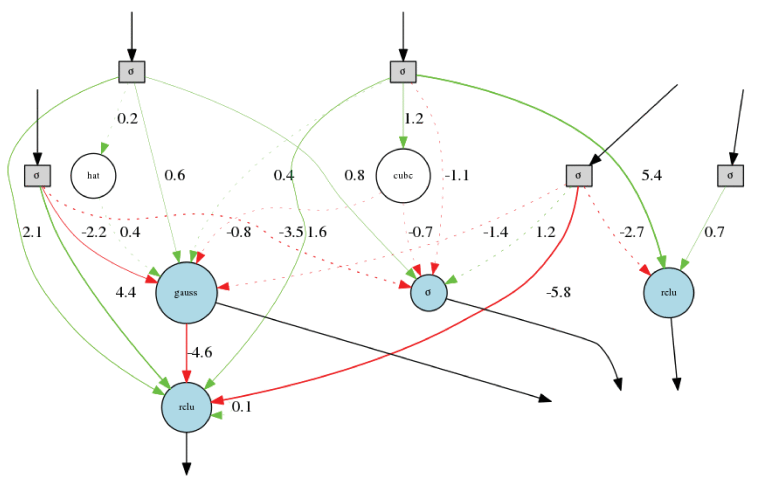
\includegraphics[width=5in]{images/tricolor-cppn.png}
    \caption{fixed-point CPPN solution found for \textit{Tricolor} morphogenesis}
    \caption*{Dotted lines indicate disabled connections. Note the two vestigial hidden layer nodes}
    \label{fig:tricolor-cppn}
\end{figure}


\section{Using convolutional neural networks}

\noindent
\textbf{Growing Neural Cellular Automata} (Mordvintsev et al., 2020) \cite{mordvintsev2020growing} is a recent paper showing how CNNs can be applied to the problem of morphogenesis, producing stable complex image patterns from a single seed state. These structures are made extremely robust to perturbation through damage-based training. \\

A 2D CA model with a Moore neighbourhood and continuous vector state variable is used.
The continuous state allows the system to learn a differentiable update rule which can be optimized through a convolutional neural network.
The model architecture defines a state with 12 hidden channels and 4 visible channels.
The visible channels include the 3 RGB values and a special $\alpha$ channel which represents the vitality of a cell.
In particular, there are 3 types of cells.
Mature cells have $\alpha > 0.1$.
Together with their neighbours, these cells are considered "living".
Neighbours of mature cells with $\alpha \leq 0.1$ are considered "growing".
All other cells are considered "dead" and have their state vector reset to $\underline{\mathbf{0}}$ at each time step.
The hidden vectors can be thought of as an opaque encoding mechanism in the cell, much like chemical concentration or electric potentials in biological cells.\\

The training pipeline features 4 key steps.
The first is \textit{perception} in which a 3x3 convolution is applied.
Two classical Sobel filters (see Figure \ref{fig:sobel} are used to estimate the partial derivative of the state vectors in the $\overrightarrow{x}$ and $\overrightarrow{y}$ directions.
These represent the cells' signalling mechanism.
The biological analogy here would be chemical gradients or electrical signal pathways.
The gradients are flattened into a vector which is fed into a neural network of multiple layers including 1x1 convolutions and ReLU activations.
The result is iteratively fed through this network for a random number of steps in the range $[64, 96]$.
At each update, a per-cell stochastic dropout is applied to simulate a random time interval between cell updates.
This is to avoid the possibly misleading assumption of global synchronisation between cells.
The pixel-wise Euclidean loss between the RGBA channels is then optimized through backpropagation-through-time. The resultant networks from this training represent candidate update rules that can induce the growth of a pattern from a single seed.\\

\begin{figure}[!h]
    \centering
    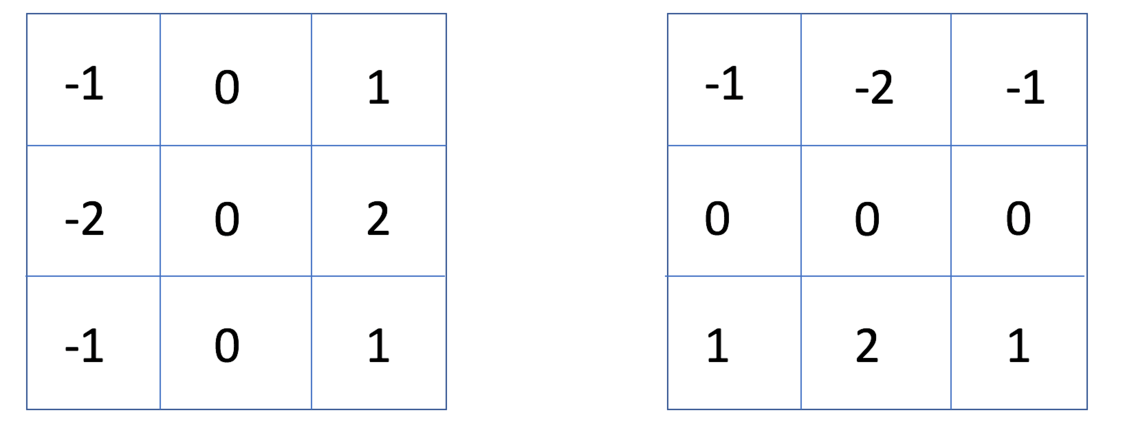
\includegraphics[width=5in]{images/sobel.png}
    \caption{Sobel filters in the x-direction (left) and y-direction (right) \cite{sodha}}
    \label{fig:sobel}
\end{figure}

However, these networks exhibited drastic instability in the long term.
To produce persistent patterns, a sample pool strategy is used whereby the network is trained on a pool of automata simultaneously.
At each step, a batch of this pool is iterated using the network.
The individual with the highest loss in the batch is reset to the seed state to prevent catastrophic forgetting \cite{mccloskey1989catastrophic}. 
Using this method, the network learns to recover from incomplete and incorrect states which makes it more likely to converge towards a persistent solution.
A simpler option to achieve persistance would've been to let the model train for longer and periodically apply a loss with exponential decaying intervals between these applications.
However, this would have drastically increased memory and training time requirements.\\

One surprising finding of this paper was that some of the resultant models exhibited regenerative behaviour when damaged, despite not being explicitly trained to do so. 
This indicates a strong overlap between solutions that exhibit persistance and those that exhibit regenerative properties. 
In order to further explore these regenerative properties, a new experiment was conducted in which a few samples in each batch were damaged before each training step. 
The system is therefore trained to recover from half-formed states.
This proved very successful. The models produced were able to grow, persist, and recover from different types of damage.\\

Overall, this paper was a very successful breakthrough in using artificial neural networks for morphogenesis. It opened up many possible areas of exploration including self-classifying CA \cite{randazzo2020self-classifying}, adversarial attacks on morphogenetic CA \cite{randazzo2021adversarial}, and learning graph CA \cite{grattarola2021learning}.

\section{Using graph neural networks}
\label{sec: using-gnn}

\noindent
\textbf{Learning Graph Cellular Automata} (Grattarola et al., 2021) \cite{grattarola2021learning} is a recent work introducing the concept of Graph Neural Cellular Automata (GNCA).
This structure extends the concept of neural cellular automata to a generalised version of CA called Graph Cellular Automata (GCA) whereby the lattice structure is replaced with an arbitrary graph.
Graph neural networks are used to learn transition rules on these GCA.\\

This paper uses two multilayer perceptrons (MLPs) connected with a message passing layer to represent the transition function for a generalised GCA.
The powerful capabilities of this simple architecture are exhibited in 3 experiments of increasing difficulty. They are:

\begin{enumerate}
  \item Voronoi: Learn a rule which flips the binary state of a cell depending on the number of living neighbours. This is analogous to Conway's Game of Life except on a Voronoi tessellation (see Figure \ref{fig:voronoi}) instead of a regular lattice. This is fairly easy since there is an explicit, known target rule and the graph topology is static. 
  \item Boids : Learn Reynold's algorithm \cite{reynolds1987flocks} to simulate the flocking of birds. This GCNA learns on a multi-agent system of points. The state of each point is a multidimensional continuous vector containing the position and velocity of each point as "visible" characteristics. This problem is more difficult. Although the target transition rule is still known, it is far more complex than the Voronoi experiment. Moreover, the graph topology is constantly changing as the points move.
  \item 3D Morphogenesis : Learn a rule for a point cloud to converge to a specified shape such that the connectivity of points has some geometrical meaning. The difficulty here arises from the fact that the target rule is unknown. This means we have little information about the attractiveness and periodicity of solutions.
\end{enumerate}

\begin{figure}[!h]
    \centering
    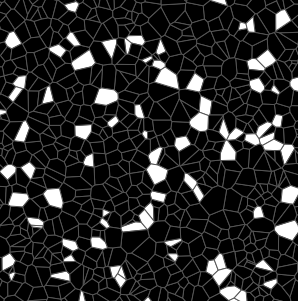
\includegraphics[width=0.5\textwidth]{images/voronoi.png}
    \caption{A GCNA learning on a Voronoi tessellation \cite{grattarola2021learning}}
    \label{fig:voronoi}
\end{figure}

This work was successful at discovering rules that can converge and persist complex target graphs including the Stanford Bunny \cite{turk} and Minnesota road network.
The key problem with the approach is that the GNCA sometimes converges to periodic solutions that orbit around the target state. 
Both fixed-point solutions and periodic solutions are class 2 CA under the Wolfram classification and, naturally, we can consider fixed-point solutions to be a subset of periodic solutions with a period of 1.
However, for the goal of producing stable shapes through morphogenesis, we are interested in discovering ways to separate these two types of solutions.
We can speculate that the model converges to periodic solutions at times because they are "close" to fixed-point solutions in the rule space.